\addcontentsline{toc}{chapter}{Занятие 4. Оценка максимального правдоподобия}
\chapter*{Занятие 4. Оценка максимального правдоподобия}

\addcontentsline{toc}{section}{Контрольные вопросы и задания}
\section*{Контрольные вопросы и задания}

\subsubsection*{Как построить оценку максимального правдоподобия?}

Плотность распределения выборки $\left( X_1, \dotsc, X_n \right) $ имеет вид
$$L \left( \vec{X}, \theta \right) =
  \prod \limits_{k = 1}^n p \left( X_k, \theta \right),$$
как плотность вектора с независимыми координатами.
$L \left( \vec{X}, \theta \right) $ --- функция правдоподобия.

Оценка максимаьлного правдоподобия $ \hat{ \theta }$ --- такое значение параметра $ \theta $,
при котором функция правдоподобия достикает своего максимального значения
$ \hat{ \theta } =
  \underset{ \theta }{argmax} L \left( \vec{X}, \theta \right) $.

\subsubsection*{Сформулируйте свойства оценки максимального правдоподобия.}

Оценка максимального правдоподобия, как правило, сильно состоятельная.

\addcontentsline{toc}{section}{Аудиторные задачи}
\section*{Аудиторные задачи}

\subsubsection*{4.6}

\textit{Задание.}
Постройте оценку максимального правдоподобия параметра $ \theta > 0$
равномерного распределения на отрезке $ \left[ 0, \theta \right] $.

\textit{Решение.}
Плотность равномерного распределения на отрезук $ \left[ 0, \theta \right] $ имеет вид
$$p_{ \theta } \left( x \right) =
  \frac{ \mathbbm{1} \left\{ x \in \left[ 0, \theta \right] \right\} }{ \theta }.$$
По этой плотности строим функцию правдоподобия
$$L \left( \vec{x}, \theta \right) =
  \frac{ \mathbbm{1} \left\{ \vec{x} \in \left[ 0, \theta \right]^n \right\} }{ \theta^n} =
  \frac{ \mathbbm{1} \left\{ \min \limits_i x_i \geq 0, \, \max \limits_i x_i \leq \theta \right\} }{ \theta^n}.$$
Если какой-то элемент выборки сильно отрицательный,
то не имеет смысла говорить о равномерном распределении, если близок к нулю,
то на него повлияла ошибка, и его не учитываем
$$ \frac{ \mathbbm{1} \left\{ \min \limits_i x_i \geq 0, \, \max \limits_i x_i \leq \theta \right\} }{ \theta^n} =
  \frac{ \mathbbm{1} \left\{ \max \limits_i x_i \leq \theta \right\} }{ \theta }.$$

Нарисуем график получившейся функции как функции от $ \theta $ (рис. \ref{fig:46}).

\begin{figure}[h!]
  \centering
  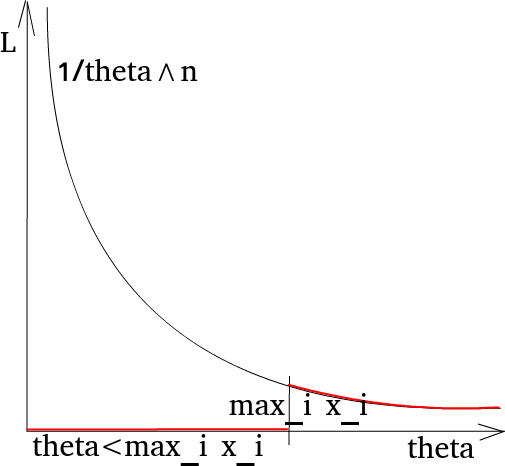
\includegraphics[width=.4\textwidth]{./pictures/4_6.png}
  \caption{График функции $L \left( \theta \right) $}
  \label{fig:46}
\end{figure}

Точка максимума такой функции --- это $ \max \limits_i x_i$.

Значит, $ \hat{ \theta } = \max \limits_{1 \leq i \leq n} x_i$.

\addcontentsline{toc}{section}{Домашнее задание}
\section*{Домашнее задание}
